\chapter{Desenvolvimento do projeto}
Neste capítulo é apresentado itens relacionados ao desenvolvimento, descrevendo as tecnologias utilizadas, escopo do projeto, dividido entre Prova de Conceito (POC)(LINK AQUI), MVP(LINK AQUI) e entrega final, arquitetura da aplicação, diagramas de modelagem e entre outros. \\
\section{Técnologias utilizadas}
As tecnologias que serão utilizadas para o desenvolvimento do aplicativo tem como o principal objetivo é deixar a aplicação flexível e viável com diferentes plataformas.\\
As ferramentas escolhidas são:
\begin{itemize}
    \item \textbf{Vscode :}
    Como IDE será usado o Vscode por sua praticidade no desenvolvimento de aplicativos e programas, além de ser super compatível com Javascript e Typescript.
    \item \textbf{JavaScript/TypeScript :}
    Como linguagem complementar do React native, além de usar o typescript para melhor estruturar o projeto no desenvolvimento.
    \item \textbf{React Native :}
    Será usado para desenvolver o aplicativo, visando atender sistemas Android e IOS de forma nativa, sendo totalmente compatível com Heroku.
    \item \textbf{Expo :}
    Consiste num conjunto de ferramentas voltadas para facilitar o desenvolvimento de aplicações mobile. Fornece diversos simplificadores para desenvolvimento e testes, sendo bem simples e prático no desenvolvimento da aplicação.
    \item \textbf{Express :}
    Como framework será utilizado o express tendo em conta que será usado Node.js na aplicação desenvolvida do projeto, e  por ser um framework minimalista e flexível.
    \item \textbf{PostgreSQL :}
    Por ser um banco de dados bem completo oferecendo a possibilidade de armazenar dados não relacionais, ele também é de fácil hospedagem no Heroku, disponibilizando a plataforma para uso gratuito em desenvolvimento.
    \item \textbf{Heroku :}
    Para a hospedagem é usado a Platform as a Service (PaaS)(LINK AQUI) Heroku, que oferece gratuitamente hospedagem que oferece para contas free 550 horas mensais de atividade de ‘app type’ (métrica de processamento da plataforma).
    \item \textbf{SVN :}
    Como uma das  ferramentas de versionamento, para gerenciar a documentação do projeto, geração de vídeos como os commits e modificações  realizadas pelos integrantes do grupo.
    \item \textbf{Docker :}
    Visando ter uma ferramenta de gerenciamento da infraestrutura aplicada será utilizado o Docker, criando uma maior agilidade na manutenção e modificação da aplicação.
    \item \textbf{Google Maps API :}
    O uso da API(LINK AQUI) do \textit{Google maps}, que disponibiliza um meio de cálculo de rotas, rastreio para acompanhar rotas, para deixar a aplicação mais completa.
\end{itemize}
    O aplicativo precisa fornecer recursos de integração com outras aplicações, isto é, autenticação utilizando API(LINK AQUI) do Google, facilitando o acesso e a criação de cadastros dos usuários.

\section{Viabilidade financeira de mantimento da aplicação}
A aplicação estará alocada no serviço de hospedagem do Heroku(LINK AQUI), que em seu plano gratuito, armazenará aplicativos não comerciais, MVPs e projetos pessoais (HEROKU, 2020)(LINK AQUI). Porém, a hospedagem é limitada, e por isso, considerando que a aplicação terá fins comerciais e futuramente será necessário aumentar a demanda de usuários, de modo que a equipe migraram para o serviço Heroku(LINK AQUI) padrão, que custa por volta de cinquenta dólares (US\$ 50) correspondente a duzentos e trinta e cinco reais e doze centavos (R\$ 235,12) mensais (HEROKU, 2020)(LINK AQUI).\\
Visando o melhor banco de dados foi identificado que o PostgreSQL(LINK AQUI) é o melhor primeiramente por ser gratuito, totalmente compatível com o Heroku(LINK AQUI), porém tendo a possibilidade de fazer doações a melhoria contínua do banco. Após o término do projeto será migrado para o plano standard com o custo de cinquenta dólares (US\$50) correspondente a duzentos e trinta e cinco reais e doze centavos (R\$235,12) mensais (HEROKU, 2020)(LINK AQUI).\\
O app será disponibilizado na Play Store(LINK AQUI) possuindo um custo fixo pago somente uma vez no valor de vinte e cinco dólares (US\$25), correspondente a cento e dezessete e cinquenta e cinco centavos  (R\$117,55 cotação atual) aproximadamente (GOOGLE PLAY CONSOLE,2022)(LINK AQUI).\\
O app também será disponibilizado na Apple Store(LINK AQUI) possuindo um custo fixo pago somente uma vez no valor de noventa e nove dólares (US\$99), correspondente a quatrocentos e sessenta e cinco reais e cinquenta e um centavos (R\$465,51 cotação atual) aproximadamente (APPLE DEVELOPER PROGRAM,2022)(LINK AQUI).\\
Para ter um maior controle da infraestrutura do projeto, agilidade de criação, manutenção e modificações de serviços o Docker(LINK AQUI) é a melhor escolha no plano gratuito, pensando em levar a aplicação adiante após a finalização do projeto, alterar o plano para o pro no valor de cinco dólares (US\$5) correspondente a vinte e tres reais e cinquenta e um centavos (R\$23,51 cotação atual) aproximadamente mensal (DOCKER,2022)(LINK AQUI)\\
Para o gerenciamento de Log, será utilizado o Papertrail(LINK AQUI), que é um software adicional no Heroku, disponibilizado no plano gratuito de dez megabytes por sete dias, porém pensando e no seguimento da aplicação, após o término do projeto, será alterado para o Plano Fixo por oito dólares (US\$8) correspondente a trinta e sete reais e vinte centavos (R\$37,20 cotação atual) aproximadamente mensal.\\
Com relação aos custos, a seguir há dois quadros que informam o custo da aplicação. O primeiro quadro (Quadro 3)(LINK AQUI) , mostra os custos durante o desenvolvimento da aplicação, também foi colocado o valor da licença da Play Store(LINK AQUI) e Apple Store(LINK AQUI) somente para ilustrar, por ser somente para o projeto a aplicação não será disponibilizada no momento.\\
O segundo quadro (Quadro 4)(LINK AQUI), informa o custo da aplicação mensal após o término do projeto, onde o grupo dá seguimento no projeto com fins lucrativos.

\newpage
\begin{figure}
    \centering
    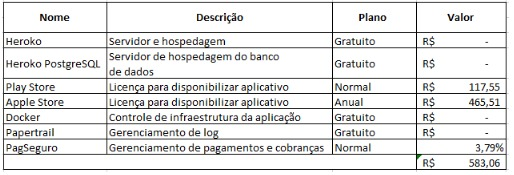
\includegraphics{exemplos/diagramas/Custo com despesas da aplicação no desenvolvimento.jpeg}
    \caption{Custo com despesas da aplicação no desenvolvimento}
    \label{fig:Custo com despesas da aplicação no desenvolvimento}
    \fonte{Os autores.}
\end{figure}\\

\begin{figure}
    \centering
    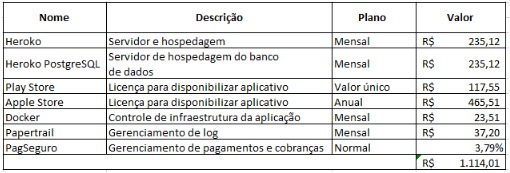
\includegraphics{exemplos/diagramas/Custo com despesas da aplicação após o término do projeto.jpeg}
    \caption{Custo com despesas da aplicação após o término do projeto}
    \label{fig:Custo com despesas da aplicação após o término do projeto}
    \fonte{Os autores.}
\end{figure}

\subsection{Captação de Receita}
Para a obtenção de fundos para a empresa e para o aplicativo, começaremos buscando parcerias, para incluir na aplicação, por esse meio, podemos fechar uma porcentagem, por indicação que pode variar de 5\% a 15\% do valor, inicialmente será variado, mas ao decorrer do tempo iremos ajustar os valores conforme o crescimento da empresa.\\
Com o tempo, prestaremos um serviço onde o parceiro poderá solicitar uma viagem em nosso aplicativo para buscar ou levar o seu animal em locais específicos, criando assim, uma parceria significativa, pois utilizaremos esse meio para ajudar a empresa terceira crescer, como também divulgaremos o nosso aplicativo para que outras empresas possam nos contratar para realizar esse tipo serviço. \\
Além das parcerias, iremos usar a opção de serviço de passeio do aplicativo para obter receita, na qual cobraremos o valor fixo de cinquenta reais (R\$50,00) a cada passeio solicitado pelo cliente. Também terá um serviço de compras dentro do aplicativo, onde forneceremos a opção do cliente disponibilizar o próprio alimento do animal ao motorista ou terá um campo específico para o cliente adicionar a compra da refeição do animal dentro do aplicativo e no final da corrida, será enviado um comprovante com os valores prestados pelo motorista. \\
E por último terá um método de viagem padrão, na qual teremos uma tarifa base de acordo com cada região, como o valor mínimo a receber, valor por minuto de viagem, valor por quilômetro rodado e o valor de serviço (do aplicativo) de 25\% que será cobrado em cada viagem ou serviço. \\
No Quadro 5(LINK AQUI) está demonstrando a cobrança da viagem padrão do passageiro e do motorista.\\

\newpage
\begin{figure}
    \centering
    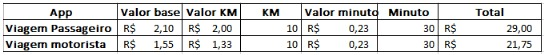
\includegraphics{exemplos/diagramas/Cálculo de viagem padrão.jpeg}
    \caption{Cálculo de viagem padrão}
    \label{fig:Cálculo de viagem padrão}
    \fonte{Os autores.}
\end{figure}\\
Para exemplificar a cobrança no quadro acima (Quadro 5)(LINK AQUI) foi realizado a fórmula: 
\mathrm{\textit{ Valor base + (Valor KM * KM) + (Valor minuto * minuto) = > Valor mínimo}}
\begin{itemize}
    \item Valor Base: é o valor fixo para se calcular a viagem;
    \item Valor KM: valor que será usado para calcular a quilometragem;
    \item KM: quilômetros percorrido na viagem;
    \item Valor Minuto: valor que será usado para calcular o minuto;
    \item Minuto: tempo de viagem em minutos;
    \item Valor Mínimo: é o valor que o motorista recebe de acordo com a região.
\end{itemize}
O cálculo acima mostrará como arrecadaremos fundos com a aplicação. \\
O Quadro 6(LINK AQUI) apresentado abaixo é o cálculo dos valores arrecadados em um dia versus a quantidade dos valores arrecadados pelo motorista em 10 horas de trabalho. \\
\newpage
\begin{figure}
    \centering
    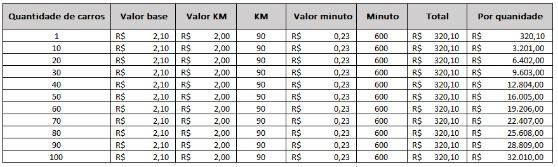
\includegraphics{exemplos/diagramas/Valor arrecadado em um dia versus quantidade de horas trabalhadas.jpeg}
    \caption{Valor arrecadado em um dia \textit{versus} quantidade de horas trabalhadas.}
    \label{fig:Valor arrecadado em um dia versus quantidade de horas trabalhadas.}
    \fonte{Os autores.}
\end{figure}\\
O Quadro 7(LINK AQUI) mostra o comparativo entre a receita mensal menos ( - ) o valor do custo mensal informado no Quadro 4(LINK AQUI).\\

\newpage
\begin{figure}
    \centering
    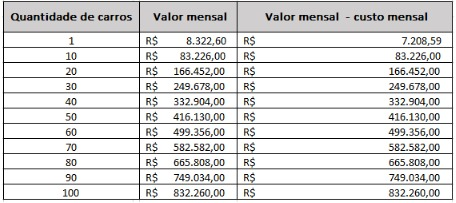
\includegraphics{exemplos/diagramas/Valor arrecadado mensal menos custo mensal.jpeg}
    \caption{Valor arrecadado mensal menos custo mensal.}
    \label{fig:Valor arrecadado mensal menos custo mensal.}
    \fonte{Os autores.}
\end{figure}\\

\section{Escopo do Projeto}
O escopo do projeto é definido para que a equipe consiga guiar as sprints e desenvolver a aplicação de maneira linear. Os itens descritos abaixo serão explicados mais adiante, na seção de requisitos funcionais, Apêndice E(LINK AQUI), requisitos não funcionais, Apêndice F(LINK AQUI) e histórias de usuários Apêndice D(LINK AQUI).

\subsection{Prova de Conceito}
A prova de conceito é utilizada para denominar um modelo prático que possa provar o conceito estabelecido neste projeto. Para a realização da POC, foi realizado o desenvolvimento do cadastro do usuário, pet e motorista e sua autenticação no sistema ao logar no Carrara Pets. 
\susection{Produto mínimo víavel (MVP)}
O MPV(LINK AQUI) define as funcionalidades essenciais para que o projeto funcione de maneira mais simples. Para isso, considera-se os itens desenvolvidos no POC(LINK AQUI) e mais alguns itens listados a seguir:
        \begin{itemize}
            \item Recuperar senha.
            \item Alterar dados cadastrados.
            \item Solicitação de transporte.
            \item Calcular tempo de viagem.
            \item Acompanhar viagem.
            \item Verificar forma de pagamento escolhida.
            \item Comparar saldo em conta com o valor da viagem.
            \item Cobrança de empresa externa para cartão.
            \item Finalizar viagem.
            \item Cancelar viagem.
            \item Avaliar viagem.
        \end{itemize}\\

\susection{Entrega Final}
Após entregar o POC(LINK AQUI) e MVP(LINK AQUI), buscamos finalizar a aplicação, seguindo o cronograma de planejamento criado no início do desenvolvimento desse projeto. Para a finalização da aplicação será necessário a inclusão de mais algumas funcionalidades, melhoria de algumas partes do desenvolvimento até o momento.
\begin{itemize}
    \item Comparar saldo em conta com o valor da viagem;
    \item Visualizar avaliações de outros usuários;
    \item Histórico de viagens;
    \item Indicação de parceiros;
    \item Catálogo de melhores motoristas por região;
    \item Personalização de fotos;
    \item Incluir valor adicional para o motorista;
    \item Criar tela de motoristas favoritos;
    \item Agendar viagens e serviços;
    \item Cobrança via cartão de crédito;
    \item Programa de pontos;
\end{itemize}\\
\section{Arquitetura da Aplicação}
Para a arquitetura do projeto foi definido a arquitetura em 3 camadas para melhor interação e controle. Por ser um método que proporciona 3 ambientes ou sistemas distintos, tornando assim o desenvolvimento mais ágil, escalabilidade mais simples e precisa, e menor possibilidade de indisponibilidade da aplicação e alto nível de segurança dos dados.\\
A arquitetura de três camadas é uma arquitetura de aplicativo de software bem estabelecida que organiza aplicativos em três camadas de computação lógica e física: a camada de apresentação ou interface do usuário; a camada do aplicativo, onde os dados são processados; e a camada de dados, em que os dados associados ao aplicativo são armazenados e gerenciados. (IBM, 2020)(LINK AQUI). Usando essa arquitetura teremos um método mais prático para escalar a aplicação, como também para trabalhar em partes específicas de modo que não prejudique a aplicação e a experiência do usuário.\\
\newpage
\begin{figure}
    \centering
    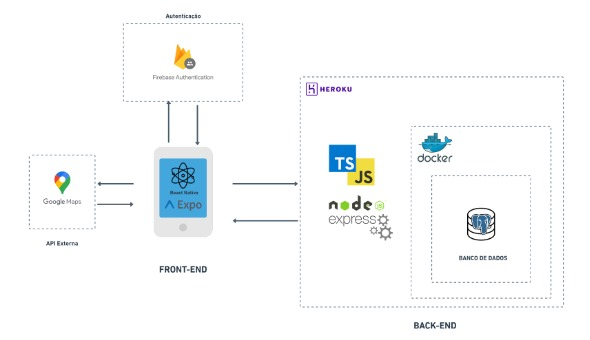
\includegraphics{exemplos/diagramas/Arquitetura Geral da Aplicação.jpeg}
    \caption{Arquitetura Geral da Aplicação}
    \label{fig:Arquitetura Geral da Aplicação}
    \fonte{Os autores.}
\end{figure}\\
Conforme o desenho da arquitetura geral, na parte do \textit{front-end(LINK AQUI)} da aplicação, teremos um sistema que rodará o \textit{Expo(LINK AQUI)} e \textit{React Native(LINK AQUI)}, desse modo, quando o cliente acessar o aplicativo abrirá a tela inicial e dará a opção de logar com a conta \textit{Google(LINK AQUI)} ou logar com a conta padrão. \\
Quando o cliente solicitar o acesso via Google, a aplicação irá acessar o \textit{Firebase(LINK AQUI)}, onde buscará junto ao \textit{Google API(LINK AQUI)} a validação da conta do cliente, e com isso, gerará um Token de validação que, devolverá o dado para o aplicativo, e por fim,  será enviado para o banco informando que o usuário estará se logando no aplicativo e salvando a informação. Diferente de quando o usuário decidir acessar com o endereço eletrônico e senha, o aplicativo levará os dados para o banco, validando a informação, e depois liberará  o acesso à conta do usuário.\\
Com o usuário dentro da aplicação, todos os dados processados do usuário serão enviados para o \textit{Docker(LINK AQUI)} avaliar, e depois será armazenado os dados no banco dentro do perfil do usuário.  \\
Como no início, a demanda será pequena, a equipe acompanhará esse processo para análise e melhoria, para diminuir o máximo possível a resposta e usabilidade da aplicação.\\

\subsection{Escalabilidade}
Escalabilidade de uma aplicação é a capacidade em que um sistema ou componente pode ser modificado para atender um ou mais problemas (GREGOL, 2011)(LINK AQUI). Atualmente, a escalabilidade deve estar sempre entre as prioridades (ENDEAVOR, 2015)(LINK AQUI), ou seja, a escalabilidade é uma característica desejada na aplicação.\\
Como um projeto é um aplicativo de transporte e tem potencial de aumento expressivo na quantidade de usuários e solicitações de acordo com seu crescimento. Por isso, é preciso da escalabilidade horizontal (GREGOL, 2011)(LINK AQUI), pois será necessário distribuir o processamento em diversas máquinas para que a aplicação responda rapidamente às requisições. Para atender essas solicitações, foi escolhido o PostgreSQL que possui a capacidade de expandir com facilidade sem perder a qualidade, de modo que agregam valor ao sistema. O Heroku(LINK AQUI), que será utilizado para escalar o sistema, limita seus recursos e serviços nos planos gratuitos, ou seja, no momento que for preciso escalar o sistema, precisará assinar planos para que possa consumir mais recursos dessas plataformas. Por isso, o Carrara Pets(LINK AQUI) usará a receita para arcar com essas despesas.\\
A necessidade de escalar o sistema provém para que a aplicação funcione de forma fluida e atenda as expectativas e satisfação dos usuários.

\section{Banco de Dados}
A aplicação tem como fonte de dados o Banco de Dados Relacional que, baseado no modelo, fornece acesso a pontos de dados relacionados entre si, possibilitando uma maneira intuitiva e direta de representar dados em tabelas. Neste modelo, cada linha na tabela é um registro com uma chave exclusiva, e suas colunas possuem atributos dos dados e cada registro. (ORACLE, 2022)(LINK AQUI). 

\section{Critérios de Segurança, Privacidade e Legislação}
    O aplicativo precisa gerenciar os dados e as informações pessoais do usuário de modo seguro, com o nível de permissão adequado(GOOGLE, 2022), visando a busca por definir medidas de manuseio e proteção dos dados dos usuários de qualquer que seja a aplicação. Será usada também a Lei Nº 13.853, implantada em 8 de julho de 2019, também chamada de Lei Geral de Proteção de Dados Pessoais (LGPD) (BRASIL, 2018).
    Como qualquer empresa séria que se preza, entende-se que os dados dos usuários e sua segurança são de extrema importância, com isso em mente, foram escolhidas as seguintes medidas de segurança:
\begin{itemize}
    \item \textbf{Senha com complexidade :} 
    O usuário na hora do cadastro no aplicativo irá solicitar que crie uma senha forte usando o padrão de no mínimo 8 dígitos com letras, números e pelo menos um caracter especial. Visando diminuir as chances de alguém adivinhar a senha, além de adicionar um limite de tentativas.
    \item \textbf{Verificação de duas etapas :} 
    Para validar e verificar a identidade do cliente, depois de se cadastrar no app é enviado um e-mail de validação para o usuário e um sms para verificar o telefone informado.
    \item \textbf{Criptografia de senha :} 
    Para a aplicação ser mais segura, será implantada a criptografia nos dados sensíveis dos clientes, como senhas, documentos dos clientes e dados bancários por meio de criptografia Hash.
\end{itemize}

\section{Critérios de LOG}
    Log é um arquivo de texto, XML e etc, que é gerado pela aplicação para descrever o seu funcionamento. Esse arquivo permite identificar problemas que podem estar ocorrendo dentro do sistema.
    Cada linha do Log contém uma informação a respeito de alguma alteração no software, ajudando a identificar falhas em requisições, respostas ou problemas nas funcionalidades do sistema.
    Para parte de logs será usado o Papertrail que é um software adicional do Heroku que analisa mensagens de log para detectar possíveis erros no sistema e disponibiliza notificações instantâneas automatizadas. 

\section{Processo de integração contínua}
    É uma prática de desenvolvimento de software em que os membros de uma equipe integram seu trabalho com frequência, geralmente cada pessoa integra pelo menos diariamente - levando a várias integrações por dia. Cada integração é verificada por uma compilação automatizada (incluindo teste) para detectar erros de integração o mais rápido possível (MARTIN , 2001).
    Para a melhoria contínua da aplicação, será utilizado o método de versionamento com o intuito de melhorar a aplicação criando melhoria de funcionalidades, correções de bugs, além de implementar novas opções e parcerias.

\section{Ferramentas para Testes automatizados e Análise Estática}
\textbf{Jest :} 
Para testes usaremos o Jest como principal framework para testes unitários e de unidade. O motivo pelo qual o escolhemos é principalmente pela sua simplicidade e facilidade de utilização e implementação.
\textbf{Testing Library :}
Também para os testes e para conseguir implementar o Jest para o mobile temos o Testing Library. Com muitas funcionalidades para facilitar a implementação e uma conversa muito boa com o Jest, esta será a nossa solução para testes.  